% !TEX root = ../Main.tex

\section{Differential Manifolds and differentiable maps}
\label{Section1}

\subsection{Review of General Topology}

Let $S$ be a set.

\begin{definition}
	A topology is a collection $\calT$ of subsets of $S$, called the open sets, such that:
	\begin{enumerate}[(i)]
		\item $\phi, S \in \calT$, where $\phi\equiv\set{}$ is the empty set.
		\item if $U_\alpha \in \calT$, for $\alpha\in A$, then $\bigcup_{\alpha\in A} U_\alpha \in \calT$
		\item if $U_1, \dots, U_n \in \calT$, $n \in \bbN$, then $\bigcap_{i=1}^n U_n \in \calT$  
	\end{enumerate}
\end{definition}

\begin{example}
	~
	\begin{enumerate}[1)]
		\item $ S=\bbR^n$, $U \in \calT$ iff $U \subseteq S$ is open in the usual sense.
		\item If $(S, d)$ is a metric space, then it is a topological space.
	\end{enumerate}
\end{example}

\begin{definition}
	Let $(S,\calT)$ be a topological space. A basis for the topology of $S$ if the collection $B \subseteq \calT$ so that any $U\in\calT$ is the union of sets from $B$.
\end{definition}

\begin{example}
	~
	\begin{enumerate}[1)]
		\item $\setst{B(x;\epsilon)}{ x \in \bbR^n, \epsilon\in\bbR^+}$ is a basis for the usual topology in $\bbR^n$.
		\item $\setst{B(x;\epsilon)}{ x \in \bbQ^n, \epsilon\in\bbQ^+}$ is a countable basis for $\bbR^n$.
	\end{enumerate}
\end{example}

\begin{definition}
	$(S,\calT)$ is second countable if the topology $\calT$ has a countable basis.
\end{definition}

\begin{definition}
	$(S,\calT)$ is Hausdorff if for all $x,y \in S$, with $x\ne y$, there are open sets $U, V \subseteq S$ so that $x \in U$, $y\in V$ and $U\cap V=\phi$.
	\begin{figure}[H]
		\centering
		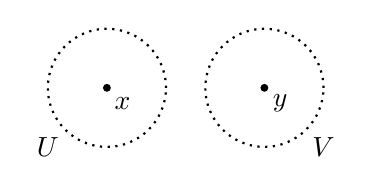
\begin{tikzpicture}
			\fill (0,0) circle(0.05) (2,0) circle(0.05);
			\draw[dotted, thick] (0,0) circle [radius=0.75] (0.2,-0.2) node {$x$} (-0.75,-0.75) node {$U$};
			\draw[dotted, thick] (2,0) circle [radius=0.75] (2.2,-0.2) node {$y$} (2.75,-0.75) node {$V$};
		\end{tikzpicture}
	\end{figure}
	In a Hausdorff space, we can always distinguish two points by enclosing them on open balls that do not intersect.
\end{definition}

Let's now define continuity in terms using topology language. Let $X, Y$ be any two topological spaces.

\begin{definition}	
	$f:X \to Y$ is continuous at $x\in X$ if for any open $V\subseteq Y$ containing $y$, there exists a open $U\subseteq X$ containing $x$ so that $f(U)\subseteq V$.
	
	\begin{figure}[H]
		\centering
			\begin{tikzpicture}
			\draw plot [smooth cycle, tension=0.5] coordinates {(-2.4,-1)(-2.8,-0)(-3.2,0.5)(-3.2,1.3)(-2.7,1.7)(-1.7,1.5)(-1.2,0.5)(-0.7,-0.5)(-1.2,-1)};
			\draw[dotted,thick, fill=green, fill opacity=0.15] (-2,0) circle(0.55);
			\draw (-1.85,-0.15) node(x) {$x$};
			\fill (-2,0) circle(0.05);
			\draw plot [smooth cycle, tension=0.5] coordinates {(1.6,-1)(0.7,0)(0.6,0.5)(0.8,1.3)(1.3,1.7)(2.7,1.5)(3.1,0.5)(3.3,-0.2)(3.1,-1)};
			\draw[dotted, thick] (2,0) circle(1.0);
			\draw[dotted, thick, fill=green, fill opacity=0.15]  plot [smooth cycle] coordinates {(1.84, -0.6)(1.48, -0.2)(1.44, 0.)(1.52, 0.32)(1.72, 0.48)(2.2, 0.4)(2.36, 0.)(2.48, -0.28)(2.4, -0.6)};
			\draw (2.15,-0.15) node(y) {$y$};
			\fill (2,0) circle(0.05);
			\node[anchor=north] at (-1.75, 0.65) (U) {};
			\node[anchor=north] at (1.70, 0.65) (fU) {};
			\draw[->,>=latex] (U) to [bend right=-30] node[above] {$f$} (fU);
			\node[below right = -0.1  and -0.1 of x] () {$U$};
			\node[above= 0.25 of y] () {$f(U)$};
			\node[below right= 0.15 and 0.2 of y] () {$V$};
			\node at (-2.5,1.4) () {$X$};
			\node at (1.8,1.4) () {$Y$};
			\end{tikzpicture}
	\end{figure} 
\end{definition}

\begin{definition}
	$f:X\to Y$ is continuous if it is continuous al all $x\in X$.
\end{definition}

\begin{proposition}
	$f:X\to Y$ is continuous iff for all open $V\subseteq Y$, the preimage $f^{-1}(V) \equiv \setst{x \in X}{ f(x) \in V} \subseteq X$ is open in $X$.	
\end{proposition}

\begin{definition}
	$F\subseteq X$ is closed if $X\backslash F \subseteq X$ is open.
\end{definition}

\begin{proposition}
	$f:X\to Y$ is continuous iff $f^{-1}(F) \subseteq X$ is closed in $X$, for every closed $F\subseteq Y$ in $Y$.
\end{proposition}

\begin{definition}
	A continuous map $f:X\to Y$ is called a homeomorphism iff it has a continuous inverse $g:Y\to X$, such that $f \circ g = \mathrm{id}_Y$ and $g \circ f = \mathrm{id}_X$. We say that $X$ and $Y$ are homeomorphic. We write $g=f^{-1}$ and $X \cong Y$. 
\end{definition}

\subsection{Differential Manifolds}

\begin{definition}
	A topological manifold of dimension $m$ is a second countable, Hausdorff topological space $M$, so that any $p \in M$ has a open neighborhood $x \ni U \subseteq M$, which is homeomorphic with $\bbR^m$.
\end{definition}

\begin{remark}
	We mightas well have said homeomorphic with an open subset of $\bbR^m$, because $B(0,\epsilon) = \setst{x\in \bbR^m}{ \norm{x} < \epsilon } \cong \bbR^m$. To see that we can use the function
	\begin{align*}
		f:~&B(0,\epsilon) \to \bbR^m \\
		& x \mapsto \frac{x}{\epsilon-\norm{x}}
	\end{align*}
\end{remark}

\begin{remark}
	The \emph{Theorem of Invariance of Domain} states that if $\phi:~\bbR^m \homeoto \bbR^n$, then $m=n$. Hence the definition is consistent.
\end{remark}



